\documentclass{standalone}
\usepackage{tikz}
\usetikzlibrary{patterns, positioning}


\begin{document}
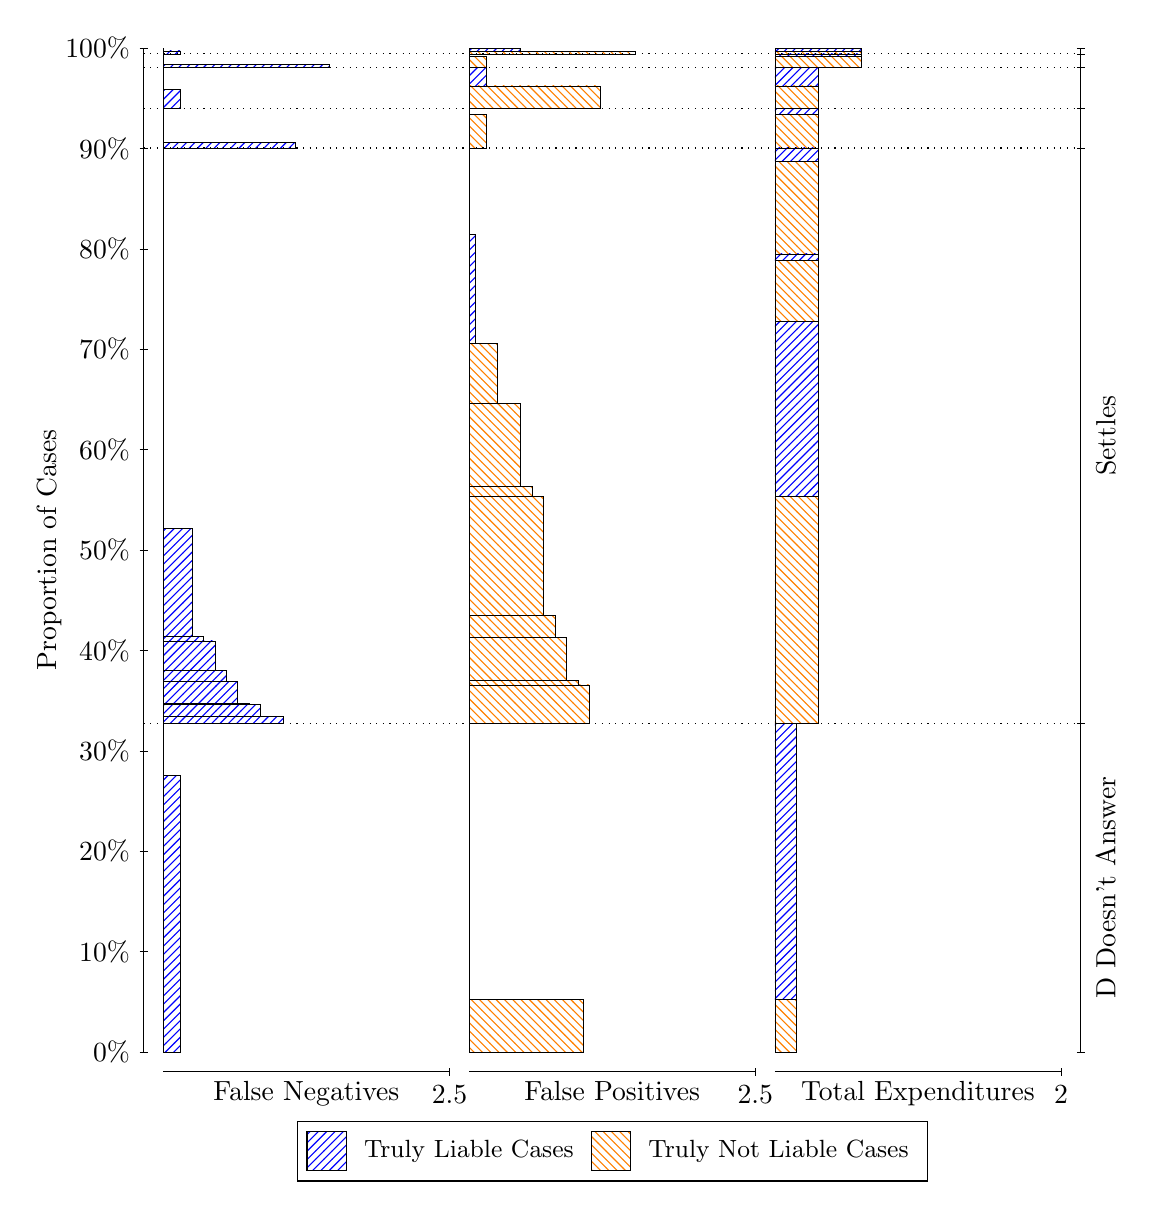
\begin{tikzpicture}
\draw[black, very thin] (1.5,1.75) -- (1.5,14.5);
\node[rotate=90, text=black, anchor=center] at (0.3, 8.125) {Proportion of Cases};
\draw[black, very thin] (1.45,1.75) -- (1.55,1.75);
\node[text=black, anchor=east] at (1.45, 1.75) {0\%};
\draw[black, very thin] (1.45,3.025) -- (1.55,3.025);
\node[text=black, anchor=east] at (1.45, 3.025) {10\%};
\draw[black, very thin] (1.45,4.3) -- (1.55,4.3);
\node[text=black, anchor=east] at (1.45, 4.3) {20\%};
\draw[black, very thin] (1.45,5.575) -- (1.55,5.575);
\node[text=black, anchor=east] at (1.45, 5.575) {30\%};
\draw[black, very thin] (1.45,6.85) -- (1.55,6.85);
\node[text=black, anchor=east] at (1.45, 6.85) {40\%};
\draw[black, very thin] (1.45,8.125) -- (1.55,8.125);
\node[text=black, anchor=east] at (1.45, 8.125) {50\%};
\draw[black, very thin] (1.45,9.4) -- (1.55,9.4);
\node[text=black, anchor=east] at (1.45, 9.4) {60\%};
\draw[black, very thin] (1.45,10.675) -- (1.55,10.675);
\node[text=black, anchor=east] at (1.45, 10.675) {70\%};
\draw[black, very thin] (1.45,11.95) -- (1.55,11.95);
\node[text=black, anchor=east] at (1.45, 11.95) {80\%};
\draw[black, very thin] (1.45,13.225) -- (1.55,13.225);
\node[text=black, anchor=east] at (1.45, 13.225) {90\%};
\draw[black, very thin] (1.45,14.5) -- (1.55,14.5);
\node[text=black, anchor=east] at (1.45, 14.5) {100\%};

\draw[black, very thin] (13.4,1.75) -- (13.4,14.5);
\draw[black, very thin] (13.35,1.75) -- (13.45,1.75);
\node[anchor=west] at (13.35, 1.75) {};
\draw[black, very thin] (13.35,5.9233) -- (13.45,5.9233);
\node[anchor=west] at (13.35, 5.9233) {};
\draw[black, very thin] (13.35,13.231) -- (13.45,13.231);
\node[anchor=west] at (13.35, 13.231) {};
\draw[black, very thin] (13.35,13.733) -- (13.45,13.733);
\node[anchor=west] at (13.35, 13.733) {};
\draw[black, very thin] (13.35,14.257) -- (13.45,14.257);
\node[anchor=west] at (13.35, 14.257) {};
\draw[black, very thin] (13.35,14.425) -- (13.45,14.425);
\node[anchor=west] at (13.35, 14.425) {};
\draw[black, very thin] (13.35,14.5) -- (13.45,14.5);
\node[anchor=west] at (13.35, 14.5) {};

\draw[black, very thin, pattern color=blue, pattern=north east lines] (1.75,1.75) rectangle (1.968,5.2581);
\draw[black, very thin, pattern color=orange, pattern=north west lines] (1.75,5.2581) rectangle (1.75,5.9233);
\draw[black, very thin, pattern color=blue, pattern=north east lines] (1.75,5.9233) rectangle (3.276,6.009);
\draw[black, very thin, pattern color=blue, pattern=north east lines] (1.75,6.009) rectangle (2.9853,6.1598);
\draw[black, very thin, pattern color=blue, pattern=north east lines] (1.75,6.1598) rectangle (2.84,6.1796);
\draw[black, very thin, pattern color=blue, pattern=north east lines] (1.75,6.1796) rectangle (2.6947,6.4551);
\draw[black, very thin, pattern color=blue, pattern=north east lines] (1.75,6.4551) rectangle (2.5493,6.6008);
\draw[black, very thin, pattern color=blue, pattern=north east lines] (1.75,6.6008) rectangle (2.404,6.9706);
\draw[black, very thin, pattern color=blue, pattern=north east lines] (1.75,6.9706) rectangle (2.2587,7.0235);
\draw[black, very thin, pattern color=blue, pattern=north east lines] (1.75,7.0235) rectangle (2.1133,8.4027);
\draw[black, very thin, pattern color=orange, pattern=north west lines] (1.75,8.4027) rectangle (1.75,13.231);
\draw[black, very thin, pattern color=blue, pattern=north east lines] (1.75,13.231) rectangle (3.4213,13.304);
\draw[black, very thin, pattern color=orange, pattern=north west lines] (1.75,13.304) rectangle (1.75,13.733);
\draw[black, very thin, pattern color=blue, pattern=north east lines] (1.75,13.733) rectangle (1.968,13.972);
\draw[black, very thin, pattern color=orange, pattern=north west lines] (1.75,13.972) rectangle (1.75,14.257);
\draw[black, very thin, pattern color=blue, pattern=north east lines] (1.75,14.257) rectangle (3.8573,14.293);
\draw[black, very thin, pattern color=orange, pattern=north west lines] (1.75,14.293) rectangle (1.75,14.425);
\draw[black, very thin, pattern color=blue, pattern=north east lines] (1.75,14.425) rectangle (1.968,14.464);
\draw[black, very thin, pattern color=orange, pattern=north west lines] (1.75,14.464) rectangle (1.75,14.5);
\draw[black, very thin, pattern color=orange, pattern=north west lines] (5.6333,1.75) rectangle (7.0867,2.4152);
\draw[black, very thin, pattern color=blue, pattern=north east lines] (5.6333,2.4152) rectangle (5.6333,5.9233);
\draw[black, very thin, pattern color=orange, pattern=north west lines] (5.6333,5.9233) rectangle (7.1593,6.4109);
\draw[black, very thin, pattern color=orange, pattern=north west lines] (5.6333,6.4109) rectangle (7.014,6.468);
\draw[black, very thin, pattern color=orange, pattern=north west lines] (5.6333,6.468) rectangle (6.8687,7.0194);
\draw[black, very thin, pattern color=orange, pattern=north west lines] (5.6333,7.0194) rectangle (6.7233,7.291);
\draw[black, very thin, pattern color=orange, pattern=north west lines] (5.6333,7.291) rectangle (6.578,8.8086);
\draw[black, very thin, pattern color=orange, pattern=north west lines] (5.6333,8.8086) rectangle (6.4327,8.9362);
\draw[black, very thin, pattern color=orange, pattern=north west lines] (5.6333,8.9362) rectangle (6.2873,9.9822);
\draw[black, very thin, pattern color=orange, pattern=north west lines] (5.6333,9.9822) rectangle (5.9967,10.751);
\draw[black, very thin, pattern color=blue, pattern=north east lines] (5.6333,10.751) rectangle (5.706,12.131);
\draw[black, very thin, pattern color=blue, pattern=north east lines] (5.6333,12.131) rectangle (5.6333,13.231);
\draw[black, very thin, pattern color=orange, pattern=north west lines] (5.6333,13.231) rectangle (5.8513,13.66);
\draw[black, very thin, pattern color=blue, pattern=north east lines] (5.6333,13.66) rectangle (5.6333,13.733);
\draw[black, very thin, pattern color=orange, pattern=north west lines] (5.6333,13.733) rectangle (7.3047,14.019);
\draw[black, very thin, pattern color=blue, pattern=north east lines] (5.6333,14.019) rectangle (5.8513,14.257);
\draw[black, very thin, pattern color=orange, pattern=north west lines] (5.6333,14.257) rectangle (5.8513,14.389);
\draw[black, very thin, pattern color=blue, pattern=north east lines] (5.6333,14.389) rectangle (5.6333,14.425);
\draw[black, very thin, pattern color=orange, pattern=north west lines] (5.6333,14.425) rectangle (7.7407,14.46);
\draw[black, very thin, pattern color=blue, pattern=north east lines] (5.6333,14.46) rectangle (6.2873,14.5);
\draw[black, very thin, pattern color=orange, pattern=north west lines] (9.5167,1.75) rectangle (9.7892,2.4152);
\draw[black, very thin, pattern color=blue, pattern=north east lines] (9.5167,2.4152) rectangle (9.7892,5.9233);
\draw[black, very thin, pattern color=orange, pattern=north west lines] (9.5167,5.9233) rectangle (10.062,8.8086);
\draw[black, very thin, pattern color=blue, pattern=north east lines] (9.5167,8.8086) rectangle (10.062,11.032);
\draw[black, very thin, pattern color=orange, pattern=north west lines] (9.5167,11.032) rectangle (10.062,11.801);
\draw[black, very thin, pattern color=blue, pattern=north east lines] (9.5167,11.801) rectangle (10.062,11.887);
\draw[black, very thin, pattern color=orange, pattern=north west lines] (9.5167,11.887) rectangle (10.062,13.06);
\draw[black, very thin, pattern color=blue, pattern=north east lines] (9.5167,13.06) rectangle (10.062,13.231);
\draw[black, very thin, pattern color=orange, pattern=north west lines] (9.5167,13.231) rectangle (10.062,13.66);
\draw[black, very thin, pattern color=blue, pattern=north east lines] (9.5167,13.66) rectangle (10.062,13.733);
\draw[black, very thin, pattern color=orange, pattern=north west lines] (9.5167,13.733) rectangle (10.062,14.019);
\draw[black, very thin, pattern color=blue, pattern=north east lines] (9.5167,14.019) rectangle (10.062,14.257);
\draw[black, very thin, pattern color=orange, pattern=north west lines] (9.5167,14.257) rectangle (10.607,14.389);
\draw[black, very thin, pattern color=blue, pattern=north east lines] (9.5167,14.389) rectangle (10.607,14.425);
\draw[black, very thin, pattern color=orange, pattern=north west lines] (9.5167,14.425) rectangle (10.607,14.46);
\draw[black, very thin, pattern color=blue, pattern=north east lines] (9.5167,14.46) rectangle (10.607,14.5);
\draw[black, dotted] (1.5,5.9233) -- (13.4,5.9233);
\draw[black, dotted] (1.5,13.231) -- (13.4,13.231);
\draw[black, dotted] (1.5,13.733) -- (13.4,13.733);
\draw[black, dotted] (1.5,14.257) -- (13.4,14.257);
\draw[black, dotted] (1.5,14.425) -- (13.4,14.425);
\draw[black, very thin] (1.75,1.5) -- (5.3833,1.5);
\node[text=black, anchor=north] at (3.5667, 1.5) {False Negatives};
\draw[black, very thin] (5.3833,1.45) -- (5.3833,1.55);
\node[text=black, anchor=north] at (5.3833, 1.45) {2.5};

\draw[black, very thin] (5.6333,1.5) -- (9.2667,1.5);
\node[text=black, anchor=north] at (7.45, 1.5) {False Positives};
\draw[black, very thin] (9.2667,1.45) -- (9.2667,1.55);
\node[text=black, anchor=north] at (9.2667, 1.45) {2.5};

\draw[black, very thin] (9.5167,1.5) -- (13.15,1.5);
\node[text=black, anchor=north] at (11.333, 1.5) {Total Expenditures};
\draw[black, very thin] (13.15,1.45) -- (13.15,1.55);
\node[text=black, anchor=north] at (13.15, 1.45) {2};

\node[text=black, centered, rotate=90] at (13.72, 3.8366) {D Doesn't Answer};
\node[text=black, centered, rotate=90] at (13.72, 9.5771) {Settles};





\draw (7.449999999999999,1.5) node[draw=none] (baseCoordinate) {};
\begin{scope}[align=center]
        \matrix[scale=0.5, draw=black, below=0.5cm of baseCoordinate, nodes={draw}, column sep=0.1cm]{
            \node[rectangle, draw, minimum width=0.5cm, minimum height=0.5cm, pattern color=blue, pattern=north east lines] {}; &
            \node[draw=none, font=\small, text=black] (B) {Truly Liable Cases}; &
            \node[rectangle, draw, minimum width=0.5cm, minimum height=0.5cm, pattern color=orange, pattern=north west lines] {}; &
            \node[draw=none, font=\small, text=black] (B) {Truly Not Liable Cases}; \\
            };
\end{scope}

\end{tikzpicture}
\end{document}